\documentclass[11pt, oneside]{article} 
\usepackage{amsmath, amsthm, amssymb, wasysym, verbatim, bbm, color, geometry}
\usepackage{amsfonts}
\usepackage{csquotes}
% \usepackage{polski}
\usepackage[english]{babel}
\usepackage[nottoc]{tocbibind}
\usepackage{caption}
\usepackage{subcaption}
\usepackage{float}
\usepackage{graphicx}
\usepackage{circuitikz}
\usepackage{listings}
\usepackage{float}
\usepackage{tikz}
\usepackage{pgfplots}

\pgfplotsset{compat=1.18}

\tikzstyle{startstop} = [rectangle, rounded corners, 
minimum width=3cm, 
minimum height=1cm,
text centered, 
draw=black, 
fill=red!30]

\tikzstyle{io} = [trapezium, 
trapezium stretches=true, % A later addition
trapezium left angle=70, 
trapezium right angle=110, 
minimum width=3cm,      
minimum height=1cm, text centered, 
rounded corners,
draw=black, fill=blue!30]

\tikzstyle{process} = [rectangle, 
minimum width=3cm, 
minimum height=1cm, 
text centered, 
text width=5cm, 
draw=black, 
rounded corners,
fill=orange!30]

\tikzstyle{decision} = [diamond, 
minimum width=3cm, 
minimum height=1cm, 
text centered, 
draw=black, 
aspect=2,
rounded corners,
fill=green!30]
\tikzstyle{arrow} = [thick,->,>=stealth]


\usetikzlibrary{shapes.geometric, arrows, arrows.meta}





\definecolor{codegreen}{rgb}{0,0.6,0}
\definecolor{codegray}{rgb}{0.5,0.5,0.5}
\definecolor{codepurple}{rgb}{0.58,0,0.82}
\definecolor{backcolour}{rgb}{0.95,0.95,0.92}

\lstdefinestyle{mystyle}{
    backgroundcolor=\color{backcolour},   
    commentstyle=\color{codegreen},
    keywordstyle=\color{magenta},
    numberstyle=\tiny\color{codegray},
    stringstyle=\color{codepurple},
    basicstyle=\ttfamily\footnotesize,
    breakatwhitespace=false,         
    breaklines=true,                 
    captionpos=b,                    
    keepspaces=true,                 
    numbers=left,                    
    numbersep=5pt,                  
    showspaces=false,                
    showstringspaces=false,
    showtabs=false,                  
    tabsize=2
}
\lstset{style=mystyle}

% \ctikzset{current arrow scale=1.5} 
\usepackage{hyperref} % Loads the hyperref package for hyperlinks
\usepackage{enumitem}
\usepackage{tikz}
\usepackage{pgfplots}
\usepackage[T1]{fontenc}
\usepackage{algorithm}
\usepackage{algpseudocode}
\usepackage{amsfonts}
\usepackage{mathbbol}

% \catcode`_=\active
% \def_#1{\sb{\mathrm{#1}}}


\pgfplotsset{compat=1.18} % Set the compatibility level for pg
\usetikzlibrary{shapes.geometric, arrows, positioning, fit, backgrounds}

\hypersetup{
    colorlinks=true,
    linkcolor=blue,
    citecolor=cyan,
    urlcolor=blue!60,
    breaklinks=true,
}





\newcommand{\workSource}[2]{Text available at: \href{#1}{#2}}



\DeclareMathSizes{12}{12}{10}{8}
\makeatletter
\renewcommand\normalsize{%
\@setfontsize\normalsize{12pt}{13.5pt}% Will look incredibly crabbed if line height is too small
\abovedisplayskip 10\p@ \@plus2\p@ \@minus5\p@%
\abovedisplayshortskip \z@ \@plus2\p@%
\belowdisplayshortskip 5\p@ \@plus2\p@ \@minus3\p@%
\belowdisplayskip \abovedisplayskip%
\let\@listi\@listI%
}
\normalsize  
\makeatother




\usepackage[style=numeric, 
            backend=biber,
           ]{biblatex}
           
\addbibresource{bibliography.bib} % Replace with your .bib file name

\geometry{tmargin=.75in, bmargin=.75in, lmargin=.75in, rmargin = .75in}  

% \usepackage{fontspec}
% \setmainfont[]{Palatino}

\newcommand{\Cdot}{\boldsymbol{\cdot}}

\newtheorem{thm}{Theorem}
\newtheorem{defn}{Definition}
\newtheorem{conv}{Convention}
\newtheorem{rem}{Remark}
\newtheorem{lem}{Lemma}
\newtheorem{cor}{Corollary}


\title{Reservoir computing}
\author{Karol Bednarz}
% \date{Rok akademicki 2024--2025}
\date{\today}



\input{constants.tex}

\begin{document}

\maketitle
\tableofcontents

\vspace{.25in}

\newcommand{\Todo}[1]{\textcolor{red}{\textbf{TODO:} #1}}

\section{Introduction}
\Todo{
    \begin{itemize}
        \item Motivation: edge AI, neuromorphic computing, in-memory computation
        \item Limitations of software RC: energy cost, latency
        \item Memristors as natural reservoir nodes: fading memory, nonlinearity, physical dynamics
        \item Gap: few hardware RC systems demonstrated end-to-end on classification tasks
        \item Contribution: physical 8x8 memristor crossbar reservoir +  MMS model + MNIST classification pipeline
        \item Paper organization
    \end{itemize}
}


\section{Background}
\Todo{
    Reservoir Computing
    \begin{itemize}
        \item RC framework: fixed reservoir, trained readout only
        \item Key properties required: echo state property, nonlinear kernel expansion
        \item Why physical substrates are attractive
    \end{itemize}
    Memristors in Neuromorphic Systems:
    \begin{itemize}
        \item Memristor fundamentals: pinched hysteresis, state equation
        \item Prior work: memristor crossbars for synaptic weights, RC, and logic
        \item Crossbar arrays: passive matrix addressing, sneak path issues
    \end{itemize}
}

\section{Memristor Device Modeling}




\Todo{
    Measurement Setup:
    \begin{itemize}
        \item Physical device description (material stack, crossbar geometry, e.g. 8x8)
        \item Characterization: I-V sweeps, pulse response, variability across cells
    \end{itemize}
    MMS Model Development:
    \begin{itemize}
        \item Model formulation: state-space representation, nonlinear dynamics
        \item Parameter extraction: from device characterization data
        \item Model validation: comparison with experimental results
    \end{itemize}
}


\subsection{Single Device Modeling with the MMS Model}

For the simulation and design of the reservoir computing system, we use Mean Metastable Switch (MMS) memristor model introduced in~\cite{Molter2016, Minati2020}. The MMS model is a simplified representation of memristor's behavior, focusing on the average switching characteristics rather than the detailed dynamics. It captures essential features of the device by describing transitions between the high-resistance state (HRS) and the low-resistance state (LRS) based on the applied voltage. This model describes memristor's dynamics as


\begin{align}
  \label{eq:mms}
  \dert{x}       & = \frac{1}{\tau} \left( f_{\rm ON}(\ua) (1-x) - f_{\rm OFF}(\ua) x \right),              \\
  f_{\rm ON}(\ua)  & = \sigma\left(-\beta (\ua-\von)\right) \label{eq:mms5b},      \\
  f_{\rm OFF}(\ua) & = 1 - \sigma\left(\beta (\ua-\voff)\right)  \label{eq:mms5c}, 
\end{align}
where \(\sigma(z) = (1+e^{-z})^{-1}\), \(\beta= \frac{q}{kT}\), \(k\) is the Boltzmann constant, \(T\) is the absolute temperature, \(q\) represents the elementary charge, while \(\von\) and \(\voff\) denote the switching voltages to LRS and HRS states, respectively. The instantaneous memductance is defined in~\eqref{eq:conductance}.

\begin{equation}
  \Gm(x) = \frac{x}{R_{\rm ON}} + \frac{1 - x}{R_{\rm OFF}},
  \label{eq:conductance}
\end{equation}

where \(\Ron\) and \(\Roff\) denote the resistances in the low-resistance and high-resistance states, respectively.


\subsection{Crossbar Array Dynamics}

Consider an \(8 \times 8\) memristor crossbar array, where each device at position \((i,j)\) is described by the MMS model with individual parameters \(\{\Ron^{(i,j)}, \Roff^{(i,j)}, \von^{(i,j)}, \voff^{(i,j)}, \tau^{(i,j)}, \beta^{(i,j)}\}\). The state of the array is given by the matrix \(\mathbf{X} \in [0,1]^{8 \times 8}\), where \(x_{ij}\) represents the internal state of the memristor at row \(i\) and column \(j\).

\paragraph{Memductance matrix.}

The conductance of each device follows from~\eqref{eq:conductance}:
\begin{equation}
  G_{ij} = \frac{x_{ij}}{R_{\rm ON}^{(i,j)}} + \frac{1 - x_{ij}}{R_{\rm OFF}^{(i,j)}}.
  \label{eq:G_matrix}
\end{equation}


\paragraph{Column voltages.}
Let \(V_{\rm row,i}(t)\) denote the voltage applied to the \(i\)-th row, and \(R_{\rm s,j}\) the series resistance at the \(j\)-th column output. The total column conductance is
\begin{equation}
  G_{\rm col,j} = \sum_{i=1}^{8} G_{ij},
  \label{eq:G_col}
\end{equation}
and the column voltage is determined by the current-divider relation
\begin{equation}
  V_{\rm col,j} = \frac{\displaystyle\sum_{i=1}^{8} V_{\rm row,i}\, G_{ij}}{G_{\rm col,j} + G_{\rm s,j}},
  \label{eq:V_col}
\end{equation}
where \(G_{\rm s,j} = 1/R_{\rm s,j}\).

\paragraph{Memristor voltage and state dynamics.}
The voltage across each memristor is
\begin{equation}
  V_{ij} = V_{\rm row,i} - V_{\rm col,j},
  \label{eq:V_mem}
\end{equation}
and its state evolves according to the MMS model~\eqref{eq:mms}:
\begin{equation}
  \dert{x_{ij}} = \frac{1}{\tau^{(i,j)}} \left( f_{\rm ON}^{(i,j)}(V_{ij})\,(1 - x_{ij}) \;-\; f_{\rm OFF}^{(i,j)}(V_{ij})\, x_{ij} \right),
  \label{eq:crossbar_dynamics}
\end{equation}
with the switching functions
\begin{align}
  f_{\rm ON}^{(i,j)}(V_{ij})  &= \sigma\!\left(-\beta^{(i,j)} (V_{ij} - V_{\rm ON}^{(i,j)})\right), \\
  f_{\rm OFF}^{(i,j)}(V_{ij}) &= 1 - \sigma\!\left(\beta^{(i,j)} (V_{ij} - V_{\rm OFF}^{(i,j)})\right).
\end{align}

The complete system consists of 64 coupled ODEs~\eqref{eq:crossbar_dynamics}, where the coupling arises through the column voltages~\eqref{eq:V_col}: each memristor's conductance \(G_{ij}\) influences \(V_{\rm col,j}\), which in turn determines the driving voltage \(V_{ij}\) for all devices in that column.



\section{Reservoir Computing System Design}


\subsection{Physical Circuit Implementation}

The proposed physical reservoir computing (RC) system is centered on an \(8 \times 8\) crossbar array of memristive devices. Within this architecture, each memristor functions as a nonlinear reservoir node, where its conductance state dynamically evolves as a function of the applied voltage and intrinsic device physics.

To facilitate bidirectional communication with the crossbar array, a dedicated peripheral analog-digital interface is employed. The signal pathways and control mechanisms are defined as follows:
\begin{itemize}
    \item \textbf{Input Interfacing:} Input data, such as pixel intensity values from the MNIST dataset, are mapped to proportional analog voltage signals using a DAC856 digital-to-analog converter (DAC). To ensure optimal signal integrity and adequate driving strength, these voltages are subsequently buffered by OPA427 operational amplifiers before being applied to the rows of the crossbar array, systematically stimulating the memristive nodes.
    \item \textbf{Output Readout:} The reservoir's state is evaluated by measuring the output currents from the crossbar columns. These currents are converted into measurable voltages via series-connected resistors. The resulting voltages are buffered by OPA427 operational amplifiers and digitized by an 8-channel 16-bit analog-to-digital converter (ADC) integrated within an STM32H755ZI microcontroller.
    \item \textbf{System Control and State Initialization:} The STM32H755ZI microcontroller serves as the central processing unit, orchestrating the input encoding, temporal synchronization, and readout harvesting. Furthermore, the circuit incorporates analog single-pole single-throw (SPST) switches to systematically reset the memristor conductance states between discrete input samples, ensuring independent transient responses for each inference cycle.
\end{itemize}


The idealized block diagram of the system is depicted in Figure~\ref{fig:block_diagram}, illustrating the interconnections between the PC, microcontroller, crossbar array, and peripheral components.


\begin{figure}[H]
    \centering
    \resizebox{0.75\textwidth}{!}{
        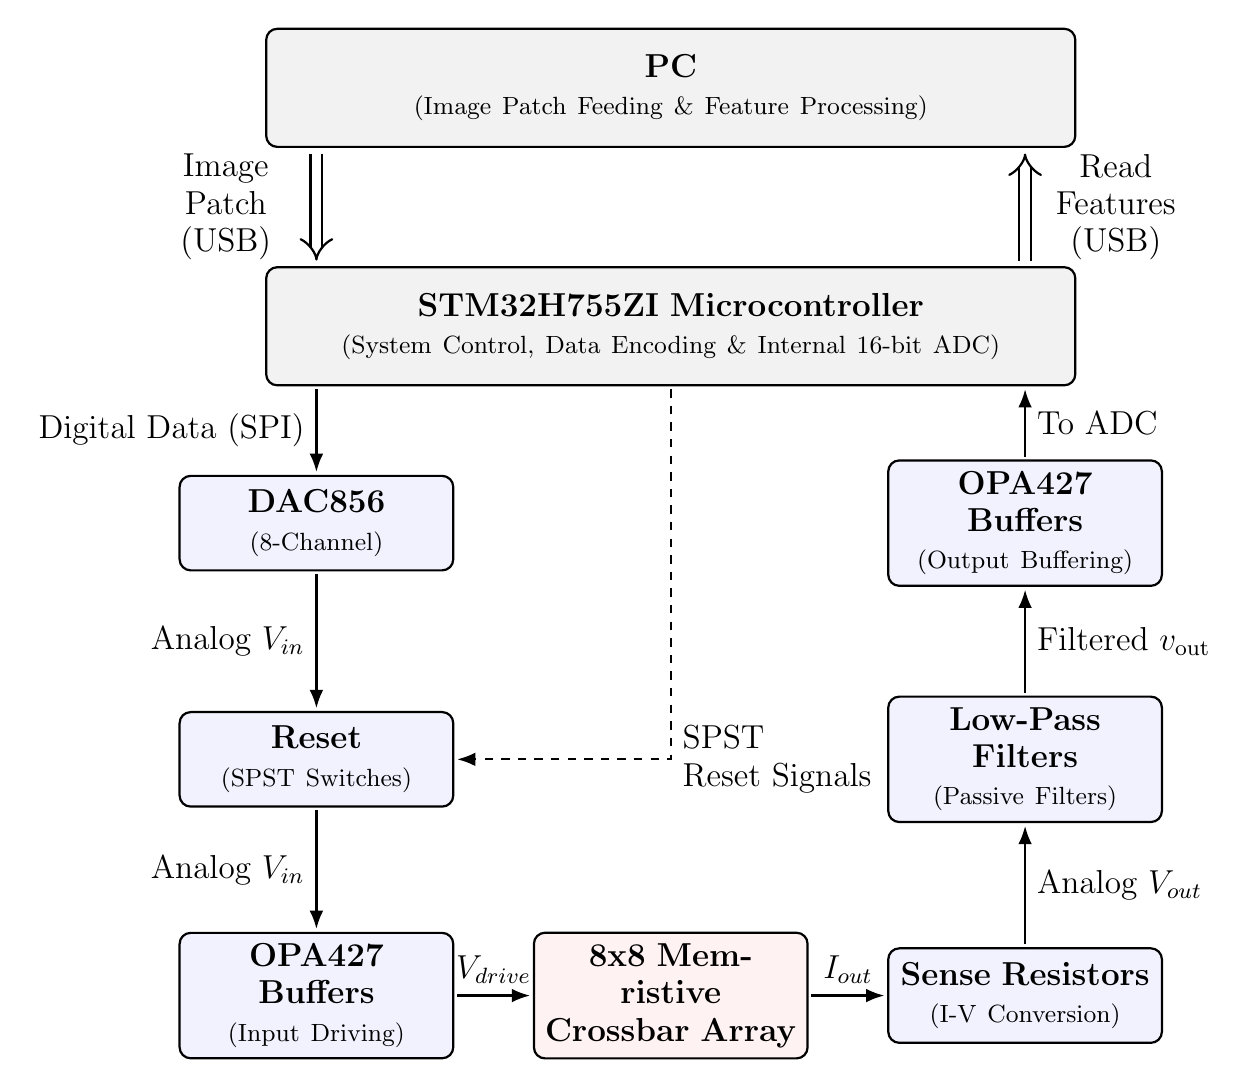
\begin{tikzpicture}[
        auto,
        block/.style = {rectangle, draw=black, thick, fill=blue!5, text width=3.2cm, align=center, rounded corners, minimum height=1.2cm},
        mcu/.style = {rectangle, draw=black, thick, fill=gray!10, text width=10cm, align=center, rounded corners, minimum height=1.5cm},
        crossbar/.style = {rectangle, draw=black, thick, fill=red!5, text width=3.2cm, align=center, rounded corners, minimum height=1.5cm},
        line/.style = {draw, thick, -Latex, shorten >=1pt, shorten <=1pt},
        doubleline/.style = {
            draw, 
            thick, 
            double, 
            double distance=3.5pt, % Slightly reduced from 5pt for a cleaner look
            -{Implies}, 
            shorten >=2pt, 
            shorten <=2pt
        }
    ]

    % --- Nodes ---
    % Microcontroller & PC (Top)
    \node [mcu] (stm) at (0,0) {\textbf{STM32H755ZI Microcontroller} \\ \small (System Control, Data Encoding \& Internal 16-bit ADC)};
    
    % Added a 1.5cm gap to prevent crowding with the STM node
    \node (pc) [mcu, above=1.5cm of stm] {\textbf{PC} \\ \small (Image Patch Feeding \& Feature Processing)}; 
    
    % Input Signal Path (Left Side)
    \node [block] (dac) at (-4.5, -2.5) {\textbf{DAC856} \\ \small (8-Channel)};
    \node [block] (switch)  at (-4.5, -5.5) {\textbf{Reset} \\ \small (SPST Switches)};
    \node [block] (inbuf) at (-4.5, -8.5) {\textbf{OPA427 Buffers} \\ \small (Input Driving)};
        
    % Reservoir Core (Center)
    \node [crossbar] (core) at (0, -8.5) {\textbf{8x8 Memristive} \\ \textbf{Crossbar Array}};
    
    % Output Readout Path (Right Side)
    \node [block] (sense) at (4.5, -8.5) {\textbf{Sense Resistors} \\ \small (I-V Conversion)};
    \node [block] (lpf) at (4.5, -5.5) {\textbf{Low-Pass Filters} \\ \small (Passive Filters)};
    \node [block] (outbuf) at (4.5, -2.5) {\textbf{OPA427 Buffers} \\ \small (Output Buffering)};

    % --- Connections ---
    % PC to STM (USB)
    \draw[doubleline] (pc.south -| dac.north) -- node[left, text width=2cm, align=center] {Image Patch\\(USB)} (stm.north -| dac.north);
    \draw[doubleline] (stm.north -| outbuf.north) -- node[right, text width=2cm, align=center] {Read Features\\(USB)} (pc.south -| outbuf.north);

    % Forward Path
    \draw [line] (stm.south -| switch.north) -- node[left] {Digital Data (SPI)} (dac.north);
    \draw [line] (dac.south) -- node[left] {Analog $V_{in}$} (switch.north);
    \draw [line] (switch.south) -- node[left] {Analog $V_{in}$} (inbuf.north);
    \draw [line] (inbuf.east) -- node[above] {$V_{drive}$} (core.west);
    
    % Readout Path
    \draw [line] (core.east) -- node[above] {$I_{out}$} (sense.west);
    \draw [line] (sense.north) -- node[right] {Analog $V_{out}$} (lpf.south);
    \draw [line] (lpf.north) -- node[right] {Filtered $v_{\mathrm{out}}$} (outbuf.south); % Changed to right and "Filtered" for clarity
    \draw [line] (outbuf.north) -- node[right] {To ADC} (stm.south -| outbuf.north);
    
    % Control/Reset Path
    % Adjusted node placement slightly to avoid crossing the digital SPI line
    \draw [line, dashed] (stm.south) |- node[right, align=left] {SPST \\ Reset Signals} (switch.east);

\end{tikzpicture}

    }
    \caption{Schematic block diagram of the memristor-based reservoir computing system. The STM32H755ZI microcontroller interfaces with the DAC and ADC to drive the crossbar array and read out the reservoir states, while the PC handles data preprocessing and readout training.}
    \label{fig:block_diagram}
\end{figure}



\Todo{
    Crossbar Reservoir Architecture
    \begin{itemize}
        \item Input encoding: voltage mapping of pixel patches / features
        \item Reservoir topology: how crossbar columns/rows act as nodes
        \item Readout: linear classifier (ridge regression or similar) on harvested currents
    \end{itemize}
    Training Protocol
    \begin{itemize}
        \item Only readout layer trained; reservoir weights fixed (physical)
        \item Dataset: MNIST preprocessing (patch extraction, normalization)
        \item Readout training: ridge regression / least-squares
    \end{itemize}
    Simulation Framework
    \begin{itemize}
        \item MMS-based SPICE or ODE simulation for design-space exploration
        \item Correspondence between simulation and hardware measurements
    \end{itemize}
}

\section{Experimental Results}
\Todo{
     Device Characterization Results - I-V curves, endurance, variability statistics \\
     MNIST Classification Performance 
     \begin{itemize}
        \item Accuracy vs. baseline (software ESN, logistic regression)
        \item Effect of reservoir size / input encoding on accuracy
        \item Confusion matrix
     \end{itemize}
     Analysis
     \begin{itemize}
        \item Role of memristive nonlinearity and fading memory in classification
        \item Impact of device-to-device variability (feature vs. bug)
     \end{itemize}
}


\section{Discussion \& Conclusion}
\Todo{
\begin{itemize}
    \item What the MMS model captures vs. misses
    \item Scalability: path from 8×8 to larger arrays
    \item Limitations: sneak paths, write endurance, thermal drift
    \item Comparison with related hardware RC systems
    \item Summary of contributions
    \item Key result (accuracy figure)
    \item Outlook: larger crossbars, online learning, spike-based input encoding
\end{itemize}
}



\printbibliography

\end{document}

